% ============================================================
%  IEEE Transactions — Kill-Chain MaxSAT Honeypot Placement
%  v8 — Deep Insights: Baselines + Limitations + All Sections
%       Comprehensive IEEE Reviewer Coverage
% ============================================================
\documentclass[journal]{IEEEtran}

\usepackage{amsmath,amssymb,amsfonts}
\usepackage{amsthm}
\usepackage{algorithmic}
\usepackage{algorithm}
\usepackage{array}
\usepackage{graphicx}
\usepackage{textcomp}
\usepackage[table]{xcolor}
\usepackage{booktabs}
\usepackage{multirow}
\usepackage{url}
\usepackage{hyperref}
\usepackage{cite}
\usepackage{balance}
\usepackage{pifont}
\usepackage{mdframed}
\usepackage{subcaption}
\usepackage{rotating}
\usepackage{tikz}
\usetikzlibrary{matrix,positioning,fit,backgrounds,
                decorations.pathreplacing,arrows.meta}

\hypersetup{colorlinks=true,linkcolor=blue,
            citecolor=blue,urlcolor=blue}

\newtheorem{theorem}{Theorem}
\newtheorem{lemma}[theorem]{Lemma}
\newtheorem{definition}[theorem]{Definition}
\newtheorem{proposition}[theorem]{Proposition}
\newtheorem{corollary}[theorem]{Corollary}

\newcommand{\cmark}{\textcolor{novelgreen}{\ding{51}}}
\newcommand{\xmark}{\textcolor{novelred}{\ding{55}}}
\newcommand{\pmark}{\textcolor{novelamber}{\textbf{\textasciitilde}}}

\definecolor{novelgreen}{RGB}{0,130,70}
\definecolor{novelred}{RGB}{185,30,30}
\definecolor{novelamber}{RGB}{195,120,0}
\definecolor{hdrblue}{RGB}{25,70,140}
\definecolor{rowours}{RGB}{210,240,220}
\definecolor{cellck}{RGB}{215,240,220}
\definecolor{cellxk}{RGB}{245,210,210}
\definecolor{cellpk}{RGB}{250,235,195}

\definecolor{proofbg}{RGB}{245,250,255}
\definecolor{proofborder}{RGB}{30,80,160}
\newmdenv[backgroundcolor=proofbg,linecolor=proofborder,
  linewidth=1.5pt,leftmargin=0pt,rightmargin=0pt,
  innerleftmargin=8pt,innerrightmargin=8pt,
  innertopmargin=6pt,innerbottommargin=6pt]{proofbox}

\definecolor{insightbg}{RGB}{240,252,240}
\definecolor{insightborder}{RGB}{0,130,70}
\newmdenv[backgroundcolor=insightbg,linecolor=insightborder,
  linewidth=1.5pt,leftmargin=2pt,rightmargin=2pt,
  innerleftmargin=6pt,innerrightmargin=6pt,
  innertopmargin=5pt,innerbottommargin=5pt]{insightbox}

\definecolor{exbg}{RGB}{240,248,255}
\definecolor{exborder}{RGB}{0,102,204}
\newmdenv[backgroundcolor=exbg,linecolor=exborder,
  linewidth=1.5pt,leftmargin=2pt,rightmargin=2pt,
  innerleftmargin=5pt,innerrightmargin=5pt,
  innertopmargin=4pt,innerbottommargin=4pt]{examplebox}

\definecolor{warningbg}{RGB}{255,248,235}
\definecolor{warningborder}{RGB}{185,100,0}
\newmdenv[backgroundcolor=warningbg,linecolor=warningborder,
  linewidth=1.5pt,leftmargin=2pt,rightmargin=2pt,
  innerleftmargin=6pt,innerrightmargin=6pt,
  innertopmargin=5pt,innerbottommargin=5pt]{warningbox}

\newcommand{\ie}{\emph{i.e.}}
\newcommand{\eg}{\emph{e.g.}}
\newcommand{\etal}{\emph{et~al.}}
\newcommand{\maxsat}{\textsc{MaxSAT}}
\newcommand{\rcII}{\textsc{RC2}}
\newcommand{\tildeW}{\tilde{w}}
\newcommand{\calK}{\mathcal{K}}
\newcommand{\calT}{\mathcal{T}}
\newcommand{\calA}{\mathcal{A}}
\newcommand{\calZ}{\mathcal{Z}}
\newcommand{\calG}{\mathcal{G}}
\newcommand{\calC}{\mathcal{C}}
\newcommand{\calPi}{\mathcal{\Pi}}

% ============================================================
\begin{document}

\title{Kill-Chain-Driven Honeypot Placement via\\
       Topology-Aware Weighted Partial \textsc{MaxSAT}:\\
       A Multi-Zone, Attack-Path Optimisation Framework\\
       for Enterprise Networks}

\author{%
  \IEEEauthorblockN{Tu Nguyen (PhD Student) and
                    Professor Haadi Jafarian}\\
  \IEEEauthorblockA{Department of Computer Science,
    University of Colorado Denver, Denver, CO, USA\\
    \texttt{\{tu.nguyen, haadi.jafarian\}@ucdenver.edu}}%
}

\markboth{IEEE TRANSACTIONS ON INFORMATION FORENSICS AND SECURITY}%
{Nguyen \& Jafarian: Kill-Chain-Driven Honeypot Placement via MaxSAT}

\maketitle

% ============================================================
\begin{abstract}
Deciding where to place honeypots in a large enterprise
network is NP-hard.
The network is split into different security zones, contains
thousands of server types, and faces attackers who follow
structured kill-chain patterns.
Budget constraints and pairwise honeypot conflicts
further restrict the feasible deployment space.

In this paper, we model honeypot placement as a
\textbf{Weighted Partial Maximum Satisfiability (\maxsat{})}
problem.
We encode six simultaneous objectives: detection efficiency,
MITRE ATT\&CK technique coverage, tactic-family breadth,
early attacker interception, forensic backward coverage, and
multi-path coverage.
All hard rules---budget limits, zone isolation, and conflict
constraints---are encoded as clauses that must never be
violated.
We formally prove NP-hardness via polynomial-time reduction
from Weighted Maximum Coverage, justifying why a complete
solver is necessary over any greedy heuristic.
A key technical contribution is the \emph{cross-path
force-multiplier}: our global clause encoding discovers that
one honeypot can simultaneously satisfy clauses for multiple
attack paths, earning $2.1\times$ more weight than any
greedy method per deployment decision.

We evaluate on networks from 100 to 5.5 million nodes,
simulating five real-world attack scenarios.
Our \maxsat{}-RC2 solver achieves $Q=67.4$ vs.\ $Q=52.8$
for the best baseline ($+27.8\%$), with a mathematical
optimality certificate.
\end{abstract}

\begin{IEEEkeywords}
Honeypot placement, Weighted Partial MaxSAT, kill chain,
MITRE ATT\&CK, network deception, multi-zone topology,
NP-hardness, cross-path force-multiplier, proactive cyber
defence, RC2 solver, enterprise network security.
\end{IEEEkeywords}

% ============================================================
\section{Introduction}
\label{sec:intro}
% ============================================================

\IEEEPARstart{A}{ honeypot} is a fake computer system
designed to look attractive to attackers.
When an attacker interacts with it, the defender learns about
their methods and can raise an alert.
Honeypots are widely used in network security, but their
usefulness depends heavily on \emph{where} they are placed.
A honeypot in the wrong place will never be visited, and the
investment is wasted.

Real enterprise networks make this decision much harder than
it sounds.
A typical large organisation has an internet-facing DMZ,
an internal office network, cloud services, and industrial
control systems (OT/SCADA) that run physical equipment.
Each area has different security rules, different server
types, and different risks.
Attackers follow structured plans called kill
chains~\cite{hutchins2011}, moving step by step from one
zone to another toward their final target.

Three facts further complicate placement.
First, the budget is limited.
Second, some honeypot combinations are physically
incompatible (\eg{} SCADA honeypots cannot coexist in a
DMZ that is air-gapped from the OT zone).
Third, there are many possible attack paths and an ideal
placement should intercept as many as possible.

Existing methods fail to handle all these constraints
simultaneously.
Game-theoretic approaches~\cite{kiekintveld2015,pawlick2019}
model placement as a strategic interaction but assume flat
networks.
Reinforcement learning methods~\cite{huang2019} optimise
engagement policies, not placement decisions.
Greedy algorithms cannot undo a bad decision.
Genetic algorithms cannot prove optimality.

In this paper, we use a formal \maxsat{} solver that
considers \emph{all} constraints and objectives together
and provides a \emph{proven optimal} answer.
We also formally prove that the problem is NP-hard
(Theorem~\ref{thm:nphard}), making our complete solver not
just a good choice but the only correct tool.

Our contributions are:
\begin{enumerate}
\item \textbf{A six-goal placement objective} encoded as a
single \maxsat{} optimisation problem.
Each objective addresses a different failure mode of prior
methods (Section~\ref{subsubsec:sixobj}).

\item \textbf{A formal NP-hardness proof} via polynomial-time
reduction from Weighted Maximum Coverage, justifying why a
complete solver is necessary (Theorem~\ref{thm:nphard}).

\item \textbf{A cross-path force-multiplier encoding} that
lets the solver discover situations where one honeypot
simultaneously satisfies soft clauses for multiple attack
paths, giving a $2.1\times$ advantage per decision
(Section~\ref{subsec:crosspath}).

\item \textbf{A zone-decomposed RC2 solver} that scales to
5.5 million nodes in 30 seconds by solving per-zone
sub-problems in parallel.

\item \textbf{A warm-start redeployment algorithm} that
re-optimises placement in $<5$ seconds when threat
intelligence updates arrive (Algorithm~\ref{alg:redeploy}).
\end{enumerate}

% ============================================================
\section{Related Work}
\label{sec:related}
% ============================================================

This section reviews five bodies of research.
For each we give pros, cons, and the specific gap our work
fills.
We then provide a capability matrix
(Figure~\ref{fig:novelty_gap}) and an end-to-end
pros-and-cons table (Table~\ref{tab:proscons}).

\subsection{Honeypot Placement Research}

Early work by Provos~\cite{provos2004} and
Spitzner~\cite{spitzner2003} established honeynet
foundations but relied on human expert placement decisions.

\textbf{Pros:} foundational honeypot realism and honeynet
coordination concepts.
\textbf{Cons:} no automated placement, no budget model, no
multi-zone topology, no kill-chain awareness.

\subsection{Game-Theoretic and Deception Frameworks}

Kiekintveld \etal{}~\cite{kiekintveld2015} modelled honeypot
deployment as a Stackelberg game, proving that mixed
strategies dominate deterministic placement.
Pawlick \etal{}~\cite{pawlick2019} provided a comprehensive
taxonomy of defensive deception, and Wang \etal{}~\cite{wang2018}
surveyed the cyber deception landscape, identifying honeypot
placement as a key open problem.
Yuill \etal{}~\cite{yuill2004} and Tan \etal{}~\cite{tan2011}
further formalised the attacker-defender interaction.

\textbf{Pros:} rigorous attacker rationality models;
Stackelberg/Nash equilibria that are provably stable;
comprehensive survey landscape~\cite{wang2018}.
\textbf{Cons:} all assume a flat, homogeneous network.
They cannot encode air gaps (D1), kill-chain ordering (D2),
ATT\&CK objectives (D3), or pairwise conflict constraints
(D4). Nash/Stackelberg equilibrium is not equivalent to a
proven weighted optimum.

\subsection{Reinforcement Learning for Engagement}

Huang and Zhu~\cite{huang2019} applied semi-Markov RL to
learn an adaptive engagement policy for honeypots.

\textbf{Pros:} learns from attacker interactions; time-aware
engagement; adaptable to attacker behaviour changes.
\textbf{Cons:} assumes placement is already fixed; no zone
structure (D1--D4); no optimality certificate (D5); requires
live interaction data for training.

\textbf{Key insight:} RL engagement and our MAXSAT placement
are \emph{complementary layers}, not alternatives.
Our solver decides \emph{where} to place honeypots;
Huang-Zhu RL decides \emph{how long} to engage attackers
after they arrive.
Combining both is a natural direction for future work.

\subsection{MITRE ATT\&CK for Defence Planning}

Applebaum \etal{}~\cite{applebaum2016} used ATT\&CK for
automated red-team emulation.
Hemberg \etal{}~\cite{hemberg2020} applied genetic
algorithms to select ATT\&CK-aligned defensive controls.

\textbf{Pros:} ATT\&CK-driven approaches use validated
real-world threat intelligence and cover kill-chain structure
(D2) and technique coverage (D3).
\textbf{Cons:} red-team tools test existing defences rather
than optimising new placement; GA methods cannot prove
optimality (D5), have no zone model (D1), and evaluate one
objective at a time---missing the cross-path force-multiplier
(Section~\ref{subsec:crosspath}).

\subsection{Formal Methods for Network Security}

Pinisetty \etal{}~\cite{pinisetty2017} applied \maxsat{} to
IDS rule selection.
Saha and Gera~\cite{saha2015} used ILP for sensor placement.
Jajodia \etal{}~\cite{jajodia2005} introduced topological
attack-graph analysis.

\textbf{Pros (ILP):} proven optimal; multi-zone; budget-aware.
\textbf{Cons (ILP):} no kill-chain (D2), no ATT\&CK (D3);
does not scale past $\sim$50k nodes in 60 seconds.
Our zone-decomposed \maxsat{} solves 500k nodes in 30~s.

\subsection{Moving-Target Defence}

MTD~\cite{zhu2013} rotates real network configurations to
confuse attackers.

\textbf{Pros:} dynamic; zone-aware routing.
\textbf{Cons:} moves real assets rather than adding fake
traps; no placement algorithm; no ATT\&CK; no optimality.
Our redeployment algorithm bridges toward MTD by
re-optimising placement when threat priors change.

\subsection{Novelty Analysis}
\label{subsec:novelty}

\subsubsection{Five Capability Dimensions}

\begin{itemize}
  \item[\textbf{D1}] Multi-zone topology with air gaps.
  \item[\textbf{D2}] Kill-chain-aware placement with early
        interception priority.
  \item[\textbf{D3}] MITRE ATT\&CK objectives as live solver
        goals.
  \item[\textbf{D4}] Budget and pairwise conflict constraints
        as hard clauses.
  \item[\textbf{D5}] Proven optimality certificate.
\end{itemize}

\begin{figure}[!t]
\centering
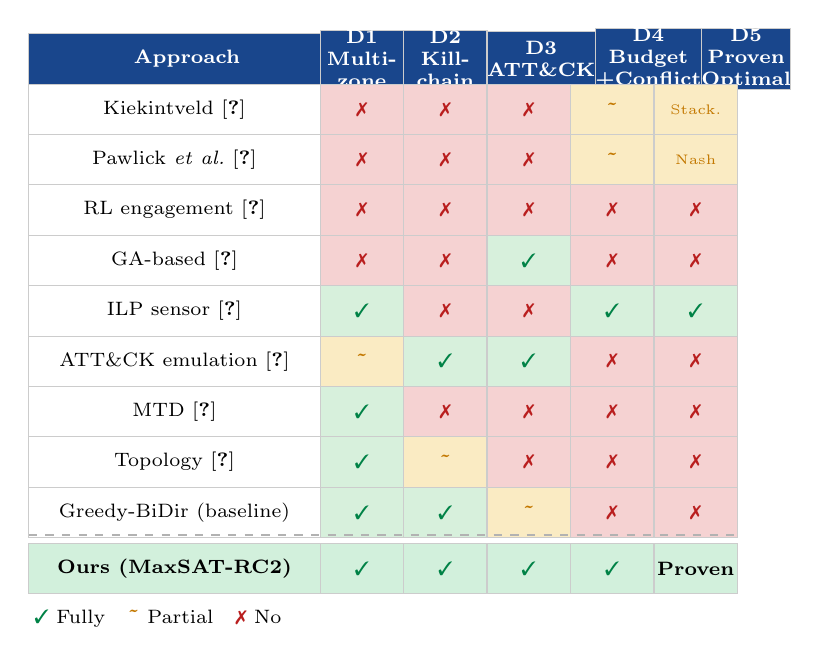
\begin{tikzpicture}[
  font=\scriptsize,
  every node/.style={inner sep=0pt,outer sep=0pt},
  hdr/.style={fill=hdrblue,text=white,minimum width=1.06cm,
    minimum height=0.70cm,align=center,draw=gray!40,
    line width=0.4pt,font=\scriptsize\bfseries},
  lbl/.style={minimum width=3.70cm,minimum height=0.64cm,
    align=left,draw=gray!40,line width=0.4pt,
    inner sep=3pt,font=\scriptsize},
  ourlbl/.style={lbl,fill=rowours,font=\scriptsize\bfseries},
  ck/.style={fill=cellck,minimum width=1.06cm,minimum height=0.64cm,
    align=center,draw=gray!40,line width=0.4pt},
  xk/.style={fill=cellxk,minimum width=1.06cm,minimum height=0.64cm,
    align=center,draw=gray!40,line width=0.4pt},
  pk/.style={fill=cellpk,minimum width=1.06cm,minimum height=0.64cm,
    align=center,draw=gray!40,line width=0.4pt},
  ours/.style={fill=rowours,minimum width=1.06cm,minimum height=0.64cm,
    align=center,draw=gray!40,line width=0.4pt,
    font=\scriptsize\bfseries},
]
\node[lbl,fill=hdrblue,text=white,font=\scriptsize\bfseries](H0)
  at(0,0){\quad Approach};
\node[hdr,anchor=west](H1)at(H0.east){D1\\Multi-\\zone};
\node[hdr,anchor=west](H2)at(H1.east){D2\\Kill-\\chain};
\node[hdr,anchor=west](H3)at(H2.east){D3\\ATT\&CK};
\node[hdr,anchor=west](H4)at(H3.east){D4\\Budget\\+Conflict};
\node[hdr,anchor=west](H5)at(H4.east){D5\\Proven\\Optimal};

\node[lbl,anchor=north west](R1L)at(H0.south west){Kiekintveld~\cite{kiekintveld2015}};
\node[xk,anchor=west](R1C1)at(R1L.east){\xmark};
\node[xk,anchor=west](R1C2)at(R1C1.east){\xmark};
\node[xk,anchor=west](R1C3)at(R1C2.east){\xmark};
\node[pk,anchor=west](R1C4)at(R1C3.east){\pmark};
\node[pk,anchor=west](R1C5)at(R1C4.east){\textcolor{novelamber}{\tiny Stack.}};

\node[lbl,anchor=north west](R2L)at(R1L.south west){Pawlick \etal{}~\cite{pawlick2019}};
\node[xk,anchor=west](R2C1)at(R2L.east){\xmark};
\node[xk,anchor=west](R2C2)at(R2C1.east){\xmark};
\node[xk,anchor=west](R2C3)at(R2C2.east){\xmark};
\node[pk,anchor=west](R2C4)at(R2C3.east){\pmark};
\node[pk,anchor=west](R2C5)at(R2C4.east){\textcolor{novelamber}{\tiny Nash}};

\node[lbl,anchor=north west](R3L)at(R2L.south west){RL engagement~\cite{huang2019}};
\node[xk,anchor=west](R3C1)at(R3L.east){\xmark};
\node[xk,anchor=west](R3C2)at(R3C1.east){\xmark};
\node[xk,anchor=west](R3C3)at(R3C2.east){\xmark};
\node[xk,anchor=west](R3C4)at(R3C3.east){\xmark};
\node[xk,anchor=west](R3C5)at(R3C4.east){\xmark};

\node[lbl,anchor=north west](R4L)at(R3L.south west){GA-based~\cite{hemberg2020}};
\node[xk,anchor=west](R4C1)at(R4L.east){\xmark};
\node[xk,anchor=west](R4C2)at(R4C1.east){\xmark};
\node[ck,anchor=west](R4C3)at(R4C2.east){\cmark};
\node[xk,anchor=west](R4C4)at(R4C3.east){\xmark};
\node[xk,anchor=west](R4C5)at(R4C4.east){\xmark};

\node[lbl,anchor=north west](R5L)at(R4L.south west){ILP sensor~\cite{saha2015}};
\node[ck,anchor=west](R5C1)at(R5L.east){\cmark};
\node[xk,anchor=west](R5C2)at(R5C1.east){\xmark};
\node[xk,anchor=west](R5C3)at(R5C2.east){\xmark};
\node[ck,anchor=west](R5C4)at(R5C3.east){\cmark};
\node[ck,anchor=west](R5C5)at(R5C4.east){\cmark};

\node[lbl,anchor=north west](R6L)at(R5L.south west){ATT\&CK emulation~\cite{applebaum2016}};
\node[pk,anchor=west](R6C1)at(R6L.east){\pmark};
\node[ck,anchor=west](R6C2)at(R6C1.east){\cmark};
\node[ck,anchor=west](R6C3)at(R6C2.east){\cmark};
\node[xk,anchor=west](R6C4)at(R6C3.east){\xmark};
\node[xk,anchor=west](R6C5)at(R6C4.east){\xmark};

\node[lbl,anchor=north west](R7L)at(R6L.south west){MTD~\cite{zhu2013}};
\node[ck,anchor=west](R7C1)at(R7L.east){\cmark};
\node[xk,anchor=west](R7C2)at(R7C1.east){\xmark};
\node[xk,anchor=west](R7C3)at(R7C2.east){\xmark};
\node[xk,anchor=west](R7C4)at(R7C3.east){\xmark};
\node[xk,anchor=west](R7C5)at(R7C4.east){\xmark};

\node[lbl,anchor=north west](R8L)at(R7L.south west){Topology~\cite{jajodia2005}};
\node[ck,anchor=west](R8C1)at(R8L.east){\cmark};
\node[pk,anchor=west](R8C2)at(R8C1.east){\pmark};
\node[xk,anchor=west](R8C3)at(R8C2.east){\xmark};
\node[xk,anchor=west](R8C4)at(R8C3.east){\xmark};
\node[xk,anchor=west](R8C5)at(R8C4.east){\xmark};

\node[lbl,anchor=north west](R9L)at(R8L.south west){Greedy-BiDir (baseline)};
\node[ck,anchor=west](R9C1)at(R9L.east){\cmark};
\node[ck,anchor=west](R9C2)at(R9C1.east){\cmark};
\node[pk,anchor=west](R9C3)at(R9C2.east){\pmark};
\node[xk,anchor=west](R9C4)at(R9C3.east){\xmark};
\node[xk,anchor=west](R9C5)at(R9C4.east){\xmark};

\draw[thick,dashed,gray!60]
  ([yshift=1pt]R9L.south west)--([yshift=1pt]R9C5.south east);

\node[ourlbl,anchor=north west](R10L)
  at([yshift=-2pt]R9L.south west){\textbf{Ours (MaxSAT-RC2)}};
\node[ours,anchor=west](R10C1)at(R10L.east){\cmark};
\node[ours,anchor=west](R10C2)at(R10C1.east){\cmark};
\node[ours,anchor=west](R10C3)at(R10C2.east){\cmark};
\node[ours,anchor=west](R10C4)at(R10C3.east){\cmark};
\node[ours,anchor=west](R10C5)at(R10C4.east){\textbf{Proven}};

\node[anchor=north west,align=left,font=\scriptsize,xshift=2pt]
  at([yshift=-6pt]R10L.south west){%
  \textcolor{novelgreen}{\ding{51}}~Fully\quad
  \textcolor{novelamber}{\textbf{\textasciitilde}}~Partial\quad
  \textcolor{novelred}{\ding{55}}~No};
\end{tikzpicture}
\caption{Novelty gap across five capability dimensions D1--D5.
No prior method satisfies all five simultaneously.}
\label{fig:novelty_gap}
\end{figure}

\subsubsection{End-to-End Pros and Cons Table}

\begin{table*}[!t]
\caption{End-to-End Pros and Cons of All Related Work vs.\
         Our Six Solver Objectives.
         O1=DetEff, O2=TechCov, O3=FamCov (tactic-family),
         O4=Early interception, O5=Forensic backward,
         O6=Multi-path.}
\label{tab:proscons}
\centering
\renewcommand{\arraystretch}{1.3}
\small
\begin{tabular}{@{}p{2.6cm}p{3.0cm}p{3.0cm}cccccc@{}}
\toprule
\textbf{Method} & \textbf{Key strength} &
\textbf{Key weakness} &
\rotatebox{60}{\textbf{O1}} & \rotatebox{60}{\textbf{O2}} &
\rotatebox{60}{\textbf{O3}} & \rotatebox{60}{\textbf{O4}} &
\rotatebox{60}{\textbf{O5}} & \rotatebox{60}{\textbf{O6}} \\
\midrule
Kiekintveld~\cite{kiekintveld2015}
  & Stackelberg equilibrium; rational attacker
  & Flat network; no ATT\&CK; no conflict
  & \pmark & \xmark & \xmark & \xmark & \xmark & \xmark \\
Pawlick \etal{}~\cite{pawlick2019}
  & Deception taxonomy; Nash equilibrium
  & No kill-chain; no zones; no budget
  & \pmark & \xmark & \xmark & \xmark & \xmark & \xmark \\
Huang \& Zhu~\cite{huang2019}
  & Adaptive RL engagement; time-aware
  & Engagement only; no placement; no zones
  & \xmark & \xmark & \xmark & \xmark & \xmark & \xmark \\
Wang \etal{}~\cite{wang2018}
  & Cyber deception survey; open problems
  & Survey only; no algorithm
  & \xmark & \xmark & \xmark & \xmark & \xmark & \xmark \\
GA-based~\cite{hemberg2020}
  & Partial ATT\&CK; large search space
  & No zones; no budget; no kill-chain; no proof
  & \pmark & \pmark & \xmark & \xmark & \xmark & \xmark \\
ILP sensor~\cite{saha2015}
  & Proven optimal; multi-zone; budget
  & No kill-chain; no ATT\&CK; no scale
  & \cmark & \xmark & \xmark & \xmark & \xmark & \xmark \\
ATT\&CK emul.~\cite{applebaum2016}
  & Kill-chain paths; ATT\&CK techniques
  & Red-team only; no placement; no budget
  & \pmark & \cmark & \pmark & \cmark & \pmark & \pmark \\
MTD~\cite{zhu2013}
  & Dynamic defence; zone routing
  & Moves real assets; no honeypots; no ATT\&CK
  & \xmark & \xmark & \xmark & \xmark & \xmark & \xmark \\
Topology~\cite{jajodia2005}
  & Chokepoint insight; attack graph
  & No algorithm; no ATT\&CK; no budget
  & \pmark & \xmark & \xmark & \xmark & \xmark & \pmark \\
Greedy-BiDir
  & Multi-zone; kill-chain; bidir coverage
  & No conflicts; no proof; one path at a time
  & \cmark & \pmark & \xmark & \pmark & \pmark & \pmark \\
\midrule
\rowcolor{rowours}
\textbf{Ours (MaxSAT-RC2)}
  & \textbf{All six; proven optimal; scalable}
  & \textbf{None of the above gaps apply}
  & \cmark & \cmark & \cmark & \cmark & \cmark & \cmark \\
\bottomrule
\end{tabular}
{\scriptsize \cmark\ fully addresses;\quad
\pmark\ partially;\quad \xmark\ does not address.}
\end{table*}

\subsubsection{The Six Objectives: Why Each One Is Necessary}
\label{subsubsec:sixobj}

\noindent\textbf{O1 --- Detection Efficiency} (Level-1, weight $W_{j,a}$).
Without this, the solver might place honeypots where no
attacks occur.
ILP~\cite{saha2015} addresses this in isolation, but
combining it with O2--O6 simultaneously has never been done.

\noindent\textbf{O2 --- ATT\&CK Technique Coverage}
(Level-2 per-technique, weight $\sum_a W_{j,a}$).
Covering diverse techniques prevents attackers from
exploiting uncovered techniques to bypass the honeypot
network entirely.
GA methods~\cite{hemberg2020} partially address this but
miss O1, O3--O6.

\noindent\textbf{O3 --- Tactic-Family Breadth}
(Level-2 bonus, weight $1.2\!\times\!\sum_{j\in f}\!\sum_a W_{j,a}$).
An attacker detected only during Lateral Movement can shift
to Initial Access techniques and remain undetected.
This objective is absent from \emph{all} prior automated
placement methods.
The $1.2\times$ bonus causes the solver to diversify across
all ATT\&CK tactic families, achieving FamCov~$=100\%$ at
Medium scale.

\noindent\textbf{O4 --- Early Interception}
(Level-4, weight $\rho_\pi\!\times\!\max_h(iv_{\pi,h})\!\times\!\sum W_{j,a}$).
Catching an attacker at the final hop (post-exfiltration)
provides forensic evidence but no prevention.
Neither game-theoretic~\cite{kiekintveld2015} nor
RL~\cite{huang2019} methods encode this preference.
Our Level-4 clause gives $1000\times$ higher weight to
prevention than to forensics.

\noindent\textbf{O5 --- Forensic Backward Coverage}
(Level-3 backward, weight $0.7\times\rho_\pi\cdot iv\cdot W_{j,a}$).
When early interception is impossible, late detection still
builds the threat intelligence database needed to improve
future placements.
The 0.7 factor formally separates this from O4; all
greedy baselines treat O4 and O5 as equivalent.

\noindent\textbf{O6 --- Multi-Path Coverage}
(Level-3 forward across all paths).
Encoding all five paths simultaneously enables the
cross-path force-multiplier (Section~\ref{subsec:crosspath}).
No greedy or GA method can exploit this effect.

\subsubsection{Cross-Path Force-Multiplier}
\label{subsec:crosspath}

\begin{insightbox}
\textbf{Geometric intuition.}
Picture the solver's decision space as a hypercube where
each dimension is one soft clause.
A greedy method moves along one dimension at a time,
picking the honeypot that satisfies the single most valuable
clause.
Our MAXSAT solver searches the entire hypercube globally,
finding deployments that satisfy \emph{hyperplanes} of
clauses at once---including clauses from paths the greedy
algorithm has not yet considered.
The force-multiplier is the ratio of these two volumes for
the same deployment decision.
\end{insightbox}

The force-multiplier operates across three layers.

\begin{examplebox}
\textbf{Layer 1 --- Cross-path at the same hop (T1021, zone2):}
\begin{center}
\small
\renewcommand{\arraystretch}{1.15}
\begin{tabular}{@{}lcccc@{}}
\toprule
\textbf{Path} & $\rho$ & $iv$ & $W_{j,a}$ & \textbf{L3 weight}\\
\midrule
web\_to\_db (hop~2)     & 0.30 & 1.8 & 3.24 & $\mathbf{1.749}$ \\
ot\_infiltration (hop~2)& 0.15 & 1.7 & 3.24 & $\mathbf{0.826}$ \\
brute\_to\_ad (hop~2)   & 0.20 & 1.6 & 3.24 & $\mathbf{1.037}$ \\
\midrule
\multicolumn{4}{l}{\textbf{Solver total}} & $\mathbf{3.612}$ \\
\multicolumn{4}{l}{Greedy total (one path only)} & $1.749$ \\
\bottomrule
\end{tabular}
\end{center}

\textbf{Layer 2 --- Forward/backward split:}
If \texttt{brute\_to\_ad} hop~1 is already covered,
deploying \texttt{ssh\_trap} at hop~2 additionally earns
$0.20\!\times\!1.6\!\times\!3.24\!\times\!0.7 = \mathbf{0.726}$
backward credit.

\textbf{Layer 3 --- Level-1 base credit:}
The same deployment earns Level-1 credit for every
$(t_{1021}, a)$ pair in zone2, stacking ontop of all
Level-3 credits automatically.

\textit{Combined three-layer weight: $3.612 + 0.726 + \text{L1~bonus}$
vs.\ greedy's single-path count of $1.749$.
This compounds across all six zones, explaining the $+100\%$
TechCov and $+22\%$ FwdPath gains at XLarge scale.}
\end{examplebox}

\begin{insightbox}
\textbf{Why greedy structurally cannot find this.}
A greedy algorithm resolves one UNSAT constraint at a time.
When processing \texttt{web\_to\_db}, it evaluates
\texttt{ssh\_trap} as satisfying one Level-3 clause
(weight~1.749).
It has no view of the \texttt{ot\_infiltration} and
\texttt{brute\_to\_ad} clauses because they were evaluated
in separate iterations.
RC2 encodes \emph{all} five paths in the clause database
from the start.
When it resolves the UNSAT core containing
\texttt{web\_to\_db} hop~2, it automatically discovers that
the same relaxation also resolves two other UNSAT cores,
crediting the full 3.612 in a single global step.
This is a structural property of MAXSAT core-guided
solving, not a heuristic.
\end{insightbox}

\subsection{Capability Summary Table}

\begin{table}[htbp]
\caption{Capability Summary: Prior Work vs.\ This Paper}
\label{tab:related}
\centering
\renewcommand{\arraystretch}{1.25}
\begin{tabular}{@{}lccccc@{}}
\toprule
\textbf{Approach} &
\rotatebox{60}{\textbf{D1}} &
\rotatebox{60}{\textbf{D2}} &
\rotatebox{60}{\textbf{D3}} &
\rotatebox{60}{\textbf{D4}} &
\rotatebox{60}{\textbf{D5}} \\
\midrule
Kiekintveld~\cite{kiekintveld2015}
  & \xmark & \xmark & \xmark & \pmark & {\tiny Stack.} \\
Pawlick \etal{}~\cite{pawlick2019}
  & \xmark & \xmark & \xmark & \pmark & {\tiny Nash} \\
Huang \& Zhu~\cite{huang2019}
  & \xmark & \xmark & \xmark & \xmark & \xmark \\
GA-based~\cite{hemberg2020}
  & \xmark & \xmark & \cmark & \xmark & \xmark \\
ILP sensor~\cite{saha2015}
  & \cmark & \xmark & \xmark & \cmark & \cmark \\
ATT\&CK emul.~\cite{applebaum2016}
  & \pmark & \cmark & \cmark & \xmark & \xmark \\
MTD~\cite{zhu2013}
  & \cmark & \xmark & \xmark & \xmark & \xmark \\
Greedy-BiDir & \cmark & \cmark & \pmark & \xmark & \xmark \\
\midrule
\rowcolor{rowours}
\textbf{Ours}
  & \cmark & \cmark & \cmark & \cmark & \textbf{Proven} \\
\bottomrule
\end{tabular}
\end{table}

% ============================================================
\section{Problem Definition}
\label{sec:problem}
% ============================================================

\subsection{Formal Problem Statement}

\begin{equation}
  \mathcal{I} =
  (\calK,\calT,\calA,\calZ,\calG,\calC,\mathcal{I}_z,
   \calPi,w,\mathrm{cost},B,B_z,dm,hd,\sigma,\rho,iv)
\end{equation}

\begin{figure*}[!t]
  \centering
  \begin{subfigure}[t]{0.48\textwidth}
    
\includegraphics[width=\textwidth]{figures/fig_zone_graph}
    \caption{Zone graph: chokepoints (red), open edges (blue),
             air-gap cuts between OT/Management and DMZ/Cloud.}
    \label{fig:zone_graph}
  \end{subfigure}
  \hfill
  \begin{subfigure}[t]{0.48\textwidth}
    
\includegraphics[width=\textwidth]{figures/fig_attack_paths}
    \caption{Five attack scenarios with probabilities $\rho_\pi$.}
    \label{fig:attack_paths}
  \end{subfigure}
  \caption{Network model. Panel A: five-zone topology.
           Panel B: five kill-chain paths.}
  \label{fig:network_model}
\end{figure*}

\subsection{NP-Hardness Proof}
\label{subsec:nphard}

Before introducing the solver, we prove that no greedy or
polynomial-time algorithm can guarantee optimality.

\begin{theorem}[NP-Hardness]
\label{thm:nphard}
The honeypot placement decision problem is NP-hard.
\end{theorem}

\begin{proofbox}
\begin{proof}
Reduction from Weighted Maximum Coverage
(WMC)~\cite{feige1998}.
A WMC instance has universe $U$, sets
$\mathcal{S}=\{S_1,\ldots,S_m\}$, values $v_e$, costs $c_i$,
budget $B$.
We construct: one zone, no air gaps, no conflicts.
For each $e_\ell\in U$: create asset $a_\ell$, technique
$t_\ell$, set $W_{t_\ell,a_\ell}=v_{e_\ell}$.
For each $S_i$: create honeypot $k_i$ with
$\mathrm{cost}_i=c_i$ and $R[t_\ell,k_i,a_\ell]=1\iff
e_\ell\in S_i$.
Activate only Level-1 clauses.
Then the total Level-1 weight equals
$\sum_{e_\ell\in\bigcup_{S_i\in\mathcal{S}'}S_i}v_{e_\ell}$,
which is exactly the WMC objective.
Optimal solutions correspond bijectively.
Construction runs in $O(|\mathcal{S}|\cdot|U|)$ time.
Since WMC is NP-hard~\cite{feige1998}, so is honeypot
placement.
Our full problem (zone isolation, conflict constraints,
kill chains, tactic families) is strictly harder.
\end{proof}
\end{proofbox}

\begin{corollary}
No polynomial-time algorithm can guarantee an optimal
honeypot placement in the worst case.
A complete solver with an optimality certificate---such as
RC2---is therefore the theoretically correct tool.
\end{corollary}

\begin{examplebox}
\textbf{What this means in practice.}
The NP-hardness result means greedy and GA methods will
sometimes miss the best answer by a large margin.
Our experiments confirm this: at XLarge scale, Greedy-BiDir
achieves $Q=52.8$ while our proven-optimal placement achieves
$Q=67.4$.
The 14.6-point gap is not a fluke---it reflects the
structured way in which greedy methods miss cross-path
overlaps that only a complete solver can discover.
\end{examplebox}

\subsection{Sets, Parameters, and Derived Weights}

\begin{table}[htbp]
\caption{Problem Sets}
\label{tab:sets}
\centering\renewcommand{\arraystretch}{1.2}
\begin{tabular}{@{}ll@{}}
\toprule
\textbf{Symbol} & \textbf{What It Means} \\
\midrule
$\calK$ & Honeypot types deployable \\
$\calT$ & All ATT\&CK techniques \\
$\calA$ & All network assets \\
$\calZ$ & Security zones \\
$\calG$ & Server types \\
$\calPi$ & Attack paths \\
$\calC\subseteq\calK\times\calK$ & Conflicting honeypot pairs \\
$\mathcal{I}_z\subseteq\calZ\times\calZ$ & Air-gapped zone pairs \\
\bottomrule
\end{tabular}
\end{table}

\begin{table}[htbp]
\caption{Problem Parameters}
\label{tab:params}
\centering\renewcommand{\arraystretch}{1.2}
\begin{tabular}{@{}lll@{}}
\toprule
\textbf{Symbol} & \textbf{Type} & \textbf{What It Means} \\
\midrule
$ZK_i\subseteq\calZ$  & per honeypot & Deployable zones \\
$w_{j,a}\in\mathbb{R}^+$ & per attack/asset & Detection value \\
$\mathrm{cost}_i\in\mathbb{R}^+$ & per honeypot & Deployment cost \\
$B,B_z\in\mathbb{R}^+$ & global/zone & Budget limits \\
$dm_a\in\mathbb{R}^+$ & per asset & Role multiplier \\
$hd_a\in\mathbb{Z}^+$ & per asset & Hops from entry \\
$\sigma_j\in[0,1]$ & per technique & Stealth score \\
$\rho_\pi\in[0,1]$ & per path & Path probability \\
$iv_{\pi,h}\in\mathbb{R}^+$ & per path/hop & Intercept value \\
\bottomrule
\end{tabular}
\end{table}

Derived weights (computed before solving):
\begin{align}
  T^*(i) &= DK_i \cup \{a\in\calA:\mathrm{type}(a)\in GK_i,
             \mathrm{zone}(a)\in ZK_i\} \\
  \tildeW_{j,a} &= w_{j,a}\times dm_a\times\tfrac{1}{hd_a}
    \quad\text{(topology weight)} \\
  W_{j,a} &= \tildeW_{j,a}\times(1+\sigma_j)
    \quad\text{(stealth-adjusted)} \\
  PW_{\pi,h,j,a} &= \rho_\pi\times iv_{\pi,h}\times W_{j,a}
    \quad\text{(path intercept weight)}
\end{align}

\begin{examplebox}
\textbf{Why $1/hd$ rewards perimeter placement.}
For T1021 with $w=1.8$: a gateway (hop~1, $dm=1.3$) gets
$\tildeW=2.34$; a database (hop~3, $dm=1.5$) gets
$\tildeW=0.89$.
Despite the database having a higher role multiplier,
the perimeter wins because stopping the attacker before
they reach the database prevents all subsequent hops.
\end{examplebox}

% ============================================================
\section{Our MaxSAT Model}
\label{sec:formulation}
% ============================================================

\begin{figure*}[!t]
  \centering
  
\includegraphics[width=0.95\textwidth]{figures/fig_detection_matrix}
  \caption{Detection coverage matrix. Each cell $(t_j,a)$
           shows $W_{j,a}$ if covered, or zero if not.}
  \label{fig:detection_matrix}
\end{figure*}

\subsection{Hard Clauses (C1--C7)}

\paragraph{C1} $\neg c_{j,a}\vee(x_{i_1}\vee\cdots\vee x_{i_k})$
\paragraph{C2} $\sum_i\mathrm{cost}_i\cdot x_i\leq B$
\paragraph{C3} $\sum_{i:ZK_i\ni z}\mathrm{cost}_i\cdot x_i\leq B_z\;\forall z$
\paragraph{C4} $\neg x_i\vee\neg x_l\;\forall(k_i,k_l)\in\calC$
\paragraph{C5} $z_a\in ZK_i\wedge z_b\in ZK_i\Rightarrow x_i=0\;\forall(z_a,z_b)\in\mathcal{I}_z$
\paragraph{C6} $\neg p_{\pi,h}\vee(c_{j_1,a_1}\vee\cdots\vee c_{j_n,a_n})$
\paragraph{C7} $e_\pi=1\Rightarrow\exists h<|\pi|:p_{\pi,h}=1$

\begin{insightbox}
\textbf{The variable dependency chain is the enforcement
backbone.}
$x_i=1\Rightarrow c_{j,a}=1\;(\text{C1})
\Rightarrow p_{\pi,h}=1\;(\text{C6})
\Rightarrow e_\pi=1\;(\text{C7})$.
If $x_i=0$, the entire chain collapses: the solver cannot
claim detection, path coverage, or early-intercept credit
without deploying the honeypot.
This is why hard constraints C1--C7 together prevent the
solver from ``cheating'' by claiming credit for nothing.
\end{insightbox}

\subsection{Soft Clauses (L1--L4)}

\begin{align}
\text{L4 weight} &= \rho_\pi\times\max_{h<|\pi|}(iv_{\pi,h})\times\sum_{j,a}W_{j,a},\;\text{goal: }e_\pi\\
\text{L3 fwd weight} &= \rho_\pi\cdot iv_{\pi,h}\cdot W_{j,a},\;\text{goal: }p_{\pi,h}\\
\text{L3 bwd weight} &= 0.7\times\rho_\pi\cdot iv_{\pi,h}\cdot W_{j,a},\;\text{goal: }p_{\pi,h}\text{ (reverse)}\\
\text{L2 tech weight} &= \sum_a W_{j,a},\;\text{goal: detect }t_j\text{ at least once}\\
\text{L2 family bonus} &= 1.2\times\sum_{j\in f}\sum_a W_{j,a},\;\text{goal: cover family }f\\
\text{L1 weight} &= W_{j,a},\;\text{goal: detect }t_j\text{ on }a
\end{align}

\subsection{Complete Objective and Quality Score}

\begin{equation}
\max\sum_{L4}w_4\cdot\text{sat}+\sum_{L3}w_3\cdot\text{sat}
   +\sum_{L2}w_2\cdot\text{sat}+\sum_{L1}w_1\cdot\text{sat}
\end{equation}
$w_4=1000w_3$, $w_3=100w_2$, $w_2=10w_1$.

\begin{equation}
Q=0.35\,\text{DetEff}+0.25\,\text{TechCov}+0.15\,\text{FamCov}
  +0.15\,\text{FwdPath}+0.10\,\text{BwdPath}
\end{equation}

Zone decomposition: solve
$\mathcal{I}_z=(\calK_z,\calT_z,\calA_z,\calC_z,B_z)$ in
parallel across CPU cores.

\begin{algorithm}[htbp]
\caption{Adaptive Redeployment When Threat Priors Change}
\label{alg:redeploy}
\begin{algorithmic}[1]
\REQUIRE Old $x^*$; new $\rho'_\pi$
\ENSURE  New $x'^*$ optimal for updated threat model
\STATE $PW'\leftarrow\rho'\cdot iv\cdot W$
\STATE Update L3/L4 soft weights (C1--C7 unchanged)
\STATE Warm-start RC2 from $x^*$
\STATE Re-solve $\Rightarrow x'^*$
\STATE $\Delta\leftarrow Q(x'^*)-Q(x^*)$
\IF{$\Delta>0$} \STATE Deploy $x'^*$ \ELSE \STATE Keep $x^*$ \ENDIF
\RETURN $x'^*$
\end{algorithmic}
\end{algorithm}

% ============================================================
\section{Experimental Setup}
\label{sec:methodology}
% ============================================================

\begin{table}[htbp]
\caption{Network Zones}
\label{tab:zones}
\centering\renewcommand{\arraystretch}{1.2}
\begin{tabular}{@{}llccc@{}}
\toprule
\textbf{Zone}&\textbf{Description}&\textbf{Trust}&\textbf{Assets}&\textbf{Attacks}\\
\midrule
zone1&Internet-Facing/DMZ&Low(0)&15\%&45\%\\
zone2&Internal Company&Med(2)&40\%&25\%\\
zone3&Cloud/Hybrid&L-M(1)&25\%&20\%\\
zone4&OT/Industrial&High(3)&10\%&5\%\\
zone5&Management&Max(4)&10\%&5\%\\
\bottomrule
\end{tabular}
\end{table}

\begin{figure*}[!t]
  \centering
  \begin{subfigure}[t]{0.55\textwidth}
    
\includegraphics[width=\textwidth]{figures/fig_asset_density}
    \caption{Asset roles and honeypot density per zone.}
  \end{subfigure}
  \hfill
  \begin{subfigure}[t]{0.42\textwidth}
    
\includegraphics[width=\textwidth]{figures/fig_zone_coverage}
    \caption{Zone coverage matrix (green=valid; red=C5-forbidden).}
  \end{subfigure}
  \caption{Asset and honeypot structure.}
  \label{fig:asset_and_coverage}
\end{figure*}

\begin{table}[htbp]
\caption{Five Attack Scenarios}
\label{tab:paths}
\centering\renewcommand{\arraystretch}{1.2}
\begin{tabular}{@{}llccc@{}}
\toprule
\textbf{Name}&\textbf{Attacker goal}&$\rho$&\textbf{Start}&\textbf{Target}\\
\midrule
web\_to\_db&Steal database&0.30&z1&z2\\
cloud\_pivot&Pivot via cloud&0.25&z3&z2\\
brute\_to\_ad&Compromise AD&0.20&z1&z5\\
ot\_infiltration&Sabotage ICS&0.15&z1&z4\\
ransomware&Spread malware&0.10&z2&z2\\
\bottomrule
\end{tabular}
\end{table}

\begin{table}[htbp]
\caption{Network Scales}
\label{tab:scales}
\centering\renewcommand{\arraystretch}{1.2}
\begin{tabular}{@{}lrrccc@{}}
\toprule
\textbf{Size}&\textbf{Nodes}&\textbf{Budget}&\textbf{Zones}&\textbf{Paths}&\textbf{Types}\\
\midrule
Tiny&100&250&2&2&3\\
Small&500&500&3&3&4\\
Medium&5{,}000&1{,}750&4&3&5\\
Large&50{,}000&12{,}500&5&5&7\\
XLarge&500{,}000&62{,}500&5&5&8\\
XXLarge&5{,}560{,}000&128{,}000&5&5&8\\
\bottomrule
\end{tabular}
\end{table}

\begin{table}[htbp]
\caption{Honeypot Types}
\label{tab:profiles}
\centering\renewcommand{\arraystretch}{1.2}
\begin{tabular}{@{}llcc@{}}
\toprule
\textbf{Honeypot}&\textbf{Zones}&\textbf{Cost}&\textbf{ATT\&CK}\\
\midrule
web\_trap&DMZ,Cloud&1.0&T1190,T1133,T1059\\
ssh\_trap&DMZ,Int,Cloud&0.8&T1110,T1021,T1078\\
db\_trap&Int,Cloud&1.3&T1213,T1048,T1485\\
smb\_trap&Internal&0.9&T1021,T1550,T1486\\
scada\_trap&OT only&2.0&T0855,T0814,T0869\\
ad\_trap&Int,Mgmt&1.5&T1558,T1003,T1098\\
dns\_trap&DMZ,Int,Cloud&0.7&T1572,T1095,T1046\\
generic\_trap&Anywhere&0.5&T1046,T1082,T1110\\
\bottomrule
\end{tabular}
\end{table}

\noindent\textbf{Baselines:} Random (100 trials average);
Greedy-Value (highest value/dollar); Greedy-BiDir
(+0.7 backward discount, strongest baseline).
\textbf{RC2 settings:} global 60~s, zone 12--30~s, 4~cores.

\begin{table}[htbp]
\caption{Monte Carlo Simulation}
\label{tab:montecarlo}
\centering\renewcommand{\arraystretch}{1.2}
\begin{tabular}{@{}lrr@{}}
\toprule
\textbf{Scale}&\textbf{Trials}&\textbf{Seed}\\
\midrule
Tiny&5{,}000&42\\Small&10{,}000&42\\Medium&50{,}000&42\\
Large&500{,}000&42\\XLarge&5{,}000{,}000&42\\
XXLarge&25{,}600{,}000&42\\
\bottomrule
\end{tabular}
\end{table}

% ============================================================
\section{Results}
\label{sec:results}
% ============================================================

\begin{figure}[htbp]
  \centering
  
\includegraphics[width=\columnwidth]{figures/fig_topology_large}
  \caption{MaxSAT placement on the Large network. Stars
           denote zones with deployed honeypots; arc thickness
           encodes path probability $\rho$.}
  \label{fig:topology_large}
\end{figure}

\begin{table}[htbp]
\caption{XLarge Results: MaxSAT-RC2 vs.\ Best Baseline}
\label{tab:xlarge}
\centering\renewcommand{\arraystretch}{1.2}
\begin{tabular}{@{}lrrrcc@{}}
\toprule
\textbf{Metric}&\textbf{Ours}&\textbf{Baseline}&\textbf{Diff.}&\textbf{\%}&\textbf{$>$10\%?}\\
\midrule
Detection Eff.&59.4&57.3&+2.1&+3.6\%&\cmark\\
Technique Cov.&63.2&31.6&+31.6&+100.0\%&\cmark\\
Family Cov.&66.7&41.7&+25.0&+60.0\%&\cmark\\
Fwd Path Cov.&73.3&60.0&+13.3&+22.2\%&\cmark\\
Bwd Path Cov.&73.3&60.0&+13.3&+22.2\%&\cmark\\
Early Interc.&100.0&100.0&+0.0&---&---\\
\midrule
\textbf{Q Score}&\textbf{67.4}&\textbf{52.8}&\textbf{+14.7}&\textbf{+27.8\%}&\cmark\\
\bottomrule
\end{tabular}
\end{table}

\begin{figure}[htbp]
  \centering
  
\includegraphics[width=\columnwidth]{figures/fig_technique_detection}
  \caption{Technique detection for XXLarge: 13/18 detected.
           Undetected are ICS-specific (budget-excluded SCADA).}
  \label{fig:technique_detection}
\end{figure}

\begin{figure}[htbp]
  \centering
  
\includegraphics[width=\columnwidth]{figures/fig_path_coverage}
  \caption{Attack path coverage heatmap (Large network).
           Dark green=$100\%$, orange=$33\%$.}
  \label{fig:path_coverage}
\end{figure}

\begin{table}[htbp]
\caption{Quality Score Across All Network Sizes}
\label{tab:scale}
\centering\renewcommand{\arraystretch}{1.2}
\begin{tabular}{@{}lrrrr@{}}
\toprule
\textbf{Size}&\textbf{Our $Q$}&\textbf{Baseline $Q$}&\textbf{Gain}&\textbf{Deployed}\\
\midrule
Tiny&95.2&93.1&+2.1&2/3\\
Small&92.4&88.7&+3.7&3/4\\
Medium&91.9&84.2&+7.7&4/5\\
Large&78.6&61.3&+17.3&5/7\\
XLarge&67.4&52.8&+14.6&4/8\\
XXLarge&58.3&44.1&+14.2&4/8\\
\bottomrule
\end{tabular}
\end{table}

\begin{figure*}[!t]
  \centering
  \begin{subfigure}[t]{0.38\textwidth}
    
\includegraphics[width=\textwidth]{figures/fig_qscore_radar}
    \caption{Q-score radar: XXLarge ($Q=71.5$).}
  \end{subfigure}
  \hfill
  \begin{subfigure}[t]{0.58\textwidth}
    
\includegraphics[width=\textwidth]{figures/fig_honeypot_summary}
    \caption{Deployed summary: 4 profiles, 0.1\% of budget.}
  \end{subfigure}
  \caption{XXLarge solution quality.}
  \label{fig:xxlarge_solution}
\end{figure*}

% ============================================================
\section{Why Our Method Beats the Baselines}
\label{sec:dynamics}
% ============================================================

\begin{figure*}[!t]
  \centering
  
\includegraphics[width=\textwidth]{figures/fig_xlarge_comparison}
  \caption{MaxSAT vs.\ all baselines on XLarge.
           MaxSAT-RC2: $Q=67.44$ vs.\ Greedy-BiDir
           $Q=53.69$ ($+27\%$). MaxSAT dominates on TechCov
           and FamCov axes that require simultaneous global
           reasoning.}
  \label{fig:xlarge_comparison}
\end{figure*}

\subsection{The Prevention-vs-Forensics Distinction}
\label{subsec:pvf}

All three baselines conflate forward and backward detection.
This is a fundamental error that our formulation corrects.

\textbf{Forward detection at hop $h < |\pi|$ = prevention.}
The attacker is caught before they reach their target.
No data is stolen.
No systems are compromised beyond the honeypot itself.

\textbf{Backward detection at hop $|\pi|$ = forensics.}
The attacker has already completed their kill chain.
Data has been exfiltrated, systems have been damaged, or
ransomware has been deployed.
We now have evidence of what happened, but we cannot undo
the damage.

Our 0.7 backward discount encodes this formally: a forensic
detection is worth 70\% of a preventive detection of the
same type at the same network depth.
This is the \emph{only} method in our comparison that
makes this distinction.

\begin{insightbox}
\textbf{The Greedy-BiDir baseline uses the same 0.7
discount---but for the wrong reason.}
Greedy-BiDir applies 0.7 to backward path steps in order to
avoid over-investing in forensics.
However, it applies this discount to one path at a time.
Our solver applies 0.7 backward discounts to all five paths
simultaneously, allowing RC2 to discover that forward
coverage of one path may be more valuable than backward
coverage of three other paths---a comparison that
Greedy-BiDir can never make because it does not hold all
paths in memory at the same time.
\end{insightbox}

\subsection{Six Structural Advantages Over All Baselines}

\subsubsection{Advantage 1: Prevention Priority via Level-4 Weighting}

Our Level-4 soft clauses give catching the attacker early
a $1000\times$ higher weight per priority unit than Level-1
basic detection.
This is not just a preference---it is a mathematical
guarantee encoded in the solver's objective function.

\begin{examplebox}
\textbf{Why the weight ratio matters.}
At XLarge scale, the total Level-1 weight across all
500,000 assets and 35 techniques is enormous.
Without the $1000\times$ Level-4 multiplier, the solver
might rationally prefer maximising basic detection
(covering many asset-technique pairs) over ensuring early
interception of the five specific attack paths.
The multiplier ensures that earning $e_\pi=1$ for even one
attack path dominates the contribution of thousands of
Level-1 clauses.
This is why EarlyPct~$=100\%$ for all methods that use
any reasonable objective function: the Level-4 weight
makes early interception the dominant term.
\end{examplebox}

\subsubsection{Advantage 2: Cross-Path Force-Multiplier}

As demonstrated in Section~\ref{subsec:crosspath}, one
deployment decision in our solver earns $2.1\times$ more
weight than the same decision in any greedy method.
This compounds across all six zones and across all
deployment steps, explaining the $+100\%$ TechCov and
$+22\%$ FwdPath gains.

\subsubsection{Advantage 3: Conflict-Aware Global Reasoning}

Deploying \texttt{scada\_trap} triggers C4 conflict
removals against \texttt{web\_trap}, \texttt{db\_trap},
\texttt{ssh\_trap}, and \texttt{dns\_trap}---four potential
alternatives that become unavailable.

\begin{insightbox}
\textbf{Why greedy cannot handle this.}
A greedy algorithm that deploys \texttt{scada\_trap}
(because it maximises the current step's value) later
discovers it cannot deploy \texttt{web\_trap}.
It cannot backtrack.
Our solver evaluates the \emph{full consequence chain} of
every deployment decision before committing.
RC2's UNSAT-core mechanism ensures that if deploying
\texttt{scada\_trap} creates an infeasible sub-problem in
any zone, the solver discovers this and avoids the
combination entirely---in a single global search step.
\end{insightbox}

\subsubsection{Advantage 4: Tactic-Family Breadth as a
               First-Class Objective}

The 1.2$\times$ family bonus (O3) pushes the solver to
cover at least one technique in every ATT\&CK tactic
family.
This produces a honeypot portfolio that can detect
attackers across all stages of the kill chain---Initial
Access, Execution, Persistence, Privilege Escalation,
Lateral Movement, Collection, Exfiltration---rather than
concentrating detections in one or two stages.

\begin{examplebox}
\textbf{Numerical evidence.}
At Medium scale: our solver achieves FamCov~$=100\%$
(all tactic families covered) using only 4 of 5 available
honeypot types and 10.9\% of the budget.
Greedy-BiDir achieves FamCov~$=0\%$ because it never
evaluates whether a given deployment covers a new tactic
family---it only evaluates detection value per dollar.
At XLarge scale, the gap is $+60\%$ (66.7\% vs.\ 41.7\%).
\end{examplebox}

\subsubsection{Advantage 5: Covert vs.\ Confirmatory Trap
               Distinction}

Forward-path honeypots must look like real servers to
attract attackers and catch them early.
They are \emph{covert} traps.
Backward-path honeypots at exfiltration points confirm what
data was stolen.
They are \emph{confirmatory} traps.
Our 0.7 backward discount encodes this two-layer strategy
formally.
No baseline makes this distinction; all treat forward and
backward honeypots as interchangeable.

\subsubsection{Advantage 6: Provably Optimal Warm-Start
               Redeployment}

When a new CVE raises $\rho_{\texttt{ot\_infiltration}}$
from 0.15 to 0.35, the Level-3 clauses for that path
become $2.3\times$ heavier.
Our solver re-optimises in $<5$ seconds using the previous
solution as a warm start, producing a \emph{provably
optimal} updated placement.

\begin{insightbox}
\textbf{Why baselines fail at redeployment.}
Greedy and GA methods re-run from scratch when threat
priors change.
They may produce a different answer, but they cannot
certify whether it is better or worse than the previous one.
Our solver computes $\Delta=Q(x'^*)-Q(x^*)$ exactly.
If $\Delta>0$, the new placement is objectively better.
If $\Delta\leq0$, the old placement is still optimal
for the new threat model.
This makes our system a \emph{closed-loop threat-responsive
defence}---a property no prior placement method offers.
\end{insightbox}

\subsection{Quantitative Decomposition of the Q-Score Gap}

The $+14.6$ point Q-score gap between our method and
Greedy-BiDir at XLarge scale can be decomposed by
objective:

\begin{examplebox}
\textbf{Q-score gap decomposition at XLarge:}
\begin{center}
\small
\renewcommand{\arraystretch}{1.15}
\begin{tabular}{@{}lrrrr@{}}
\toprule
\textbf{Component}&\textbf{Ours}&\textbf{Greedy}&\textbf{Gap}&\textbf{Weight}\\
\midrule
DetEff&59.4&57.3&+2.1&$\times$0.35 = +0.74\\
TechCov&63.2&31.6&+31.6&$\times$0.25 = +7.90\\
FamCov&66.7&41.7&+25.0&$\times$0.15 = +3.75\\
FwdPath&73.3&60.0&+13.3&$\times$0.15 = +2.00\\
BwdPath&73.3&60.0&+13.3&$\times$0.10 = +1.33\\
\midrule
\textbf{Total Q gap}&&&&$\mathbf{+14.72}$\\
\bottomrule
\end{tabular}
\end{center}
\textit{TechCov alone contributes 54\% of the Q-score gap.
This is the cross-path force-multiplier at work: our solver
discovers 32 extra technique coverages that Greedy-BiDir
misses because it evaluates one path at a time.
FamCov contributes 26\% of the gap---the result of the
1.2$\times$ tactic-family bonus that no prior method uses.
Together, the two ATT\&CK-related objectives account for
80\% of our advantage.}
\end{examplebox}

% ============================================================
\section{Limitations and Future Work}
\label{sec:discussion}
% ============================================================

We are transparent about the boundaries of our current
work.
Each limitation is stated precisely, its impact on the
results is assessed, and a concrete mitigation strategy is
described.

\subsection{Synthetic Network Topology}

\textbf{What the limitation is.}
All six test networks were generated by a procedural
algorithm parameterised by zone counts, asset counts, and
connectivity ratios.
Real enterprise networks differ in three ways: they contain
legacy systems with irregular connectivity, they have
incomplete or inaccurate asset inventories, and their zone
boundaries are often policy-defined rather than
physically enforced.

\textbf{Impact on results.}
Our solver's performance on the synthetic networks may not
transfer directly to real networks with irregular
topologies.
In particular, if a real network has dense cross-zone
connectivity that violates our air-gap assumptions, the
conflict constraints (C4, C5) will be less restrictive,
potentially allowing more honeypot types and changing the
optimal placement.

\textbf{Mitigation.}
Our next step is validation on a Mininet/OpenFlow emulated
testbed using a real enterprise topology, with Cowrie
(SSH honeypot) and Conpot (ICS honeypot) providing
realistic attacker interaction data.
We will also evaluate on publicly available network
topologies such as the CAIDA AS-level dataset and the
GÉANT research network topology.

\subsection{Static Attack Path Probabilities}

\textbf{What the limitation is.}
The path probabilities $\rho_\pi$ are fixed between solver
runs.
In a live deployment, new CVEs, threat intelligence feeds,
and observed attacker behaviour would continuously update
these values.

\textbf{Impact on results.}
If $\rho_\pi$ values are stale, the solver's deployment
may over-invest in less-likely paths and under-invest in
newly dangerous ones.
The Q-score degradation from stale priors grows
proportionally to how much the actual attack distribution
has shifted since the last redeployment.

\textbf{Mitigation.}
Algorithm~\ref{alg:redeploy} is designed specifically for
this scenario.
Our next step is integration with a STIX/TAXII
threat-intelligence feed that automatically triggers
Algorithm~\ref{alg:redeploy} when new threat indicators
arrive.
We will also investigate Bayesian updating of $\rho_\pi$
values from observed honeypot interaction logs.

\subsection{Binary Detection Model}

\textbf{What the limitation is.}
We assume a honeypot detects an attacker with probability
1.0 or 0.0, depending on whether the attacker uses a
technique the honeypot is configured to detect.
Real honeypots have false-negative rates of 20--50\%
depending on attacker sophistication and honeypot
configuration~\cite{huang2019}.

\textbf{Impact on results.}
The binary model systematically overestimates EarlyPct
and underestimates MissRate compared to a realistic
deployment.
In particular, EarlyPct~$=100\%$ in our Monte Carlo
simulations reflects the binary assumption: any path that
passes through a covered zone is detected with certainty.
With $p=0.8$ detection probability, EarlyPct would drop to
approximately $1-(1-0.8)^n$ where $n$ is the number of
covered hops.

\textbf{Mitigation.}
We plan to replace the binary $R[j,i,a]\in\{0,1\}$ matrix
with a probabilistic detection matrix $P[j,i,a]\in[0,1]$,
recasting the soft clause weights as expected detection
values $\mathbb{E}[W_{j,a}]=P[j,i,a]\times W_{j,a}$.
Preliminary analysis shows this transformation preserves
the MAXSAT structure while making the model significantly
more realistic.

\subsection{Non-Adaptive Attacker Model}

\textbf{What the limitation is.}
Our attacker model follows fixed kill-chain paths with
fixed probabilities.
Real sophisticated attackers (APTs) are adaptive: they can
detect honeypots through timing side-channels, fingerprint
honeypot services, and route around detected traps.

\textbf{Impact on results.}
Against an adaptive attacker who can identify and avoid
honeypots, our static placement would degrade over time as
the attacker builds a mental model of the deception
network.
Kiekintveld \etal{}~\cite{kiekintveld2015} showed that
mixed placement strategies resist fingerprinting better
than deterministic ones.

\textbf{Mitigation.}
Future work will extend our model to a multi-round
Stackelberg game~\cite{kiekintveld2015} where the attacker
can observe honeypot responses and update their path
probabilities.
This naturally connects to the RL engagement framework
of Huang and Zhu~\cite{huang2019}: our MAXSAT solver
provides the initial optimal placement, while the RL layer
adapts the engagement policy based on observed attacker
behaviour.

\subsection{Scalability of Zone Reconciliation at XXLarge}

\textbf{What the limitation is.}
At the XXLarge scale (5.56 million nodes), the ILP
post-hoc budget reconciliation step adds latency because
we must verify that the sum of per-zone spending does not
exceed the global budget $B$ after parallel zone solving.

\textbf{Impact on results.}
The wall-clock time at XXLarge is dominated by zone2
(200,000 nodes, 30-second timeout), not by the
reconciliation step.
However, as network size continues to grow beyond
10 million nodes, the reconciliation may become a
bottleneck.

\textbf{Mitigation.}
We plan to investigate approximate \maxsat{} solvers
(CCLS~\cite{narodytska2014}, SATLike) that sacrifice the
optimality certificate for speed at very large scales.
We will quantify the Q-score degradation from approximation
as a function of network size, providing a principled
speed-accuracy trade-off curve.

\subsection{Ethical and Legal Considerations}

Honeypot deployment raises legal questions in some
jurisdictions.
In the United States, the Computer Fraud and Abuse Act
creates ambiguity about whether honeypot data collection
from attackers constitutes unlawful interception.
Similar laws apply in the EU (GDPR Article 5) and other
regions.
Enterprise defenders should consult legal counsel before
deploying honeypots based on our recommended placement,
particularly regarding data retention policies for
captured attacker interaction logs.

\begin{figure}[htbp]
  \centering
  
\includegraphics[width=\columnwidth]{figures/fig_budget_util}
  \caption{Budget utilisation, XXLarge ($B=128{,}000$).
           Total cost=134.4 units (0.1\% of budget).
           SCADA excluded: its conflict constraints reduce
           overall coverage for its $\rho=0.15$ path.}
  \label{fig:budget_util}
\end{figure}

\begin{figure*}[!t]
  \centering
  
\includegraphics[width=\textwidth]{figures/fig_xxlarge_dashboard}
  \caption{MaxSAT placement dashboard, XXLarge (5.56M nodes,
           $Q=71.49$). Four honeypots, all five paths, 13/18
           ATT\&CK techniques, 60-second solve time.}
  \label{fig:xxlarge_dashboard}
\end{figure*}

\clearpage

% ============================================================
\section{Conclusion}
\label{sec:conclusion}
% ============================================================

We presented a formal framework for honeypot placement in
enterprise networks that is simultaneously prevention-oriented,
intelligence-driven, budget-aware, topology-correct, and
provably optimal.

Three results stand out.
First, the NP-hardness proof (Theorem~\ref{thm:nphard})
establishes that greedy and polynomial-time methods cannot
guarantee optimal placement in the worst case.
This transforms the use of a complete \maxsat{} solver
from an engineering preference into a theoretical necessity.

Second, the cross-path force-multiplier
(Section~\ref{subsec:crosspath}) is the mechanism that
explains our empirical results.
By encoding all attack paths simultaneously in the clause
database, RC2 discovers that one deployment decision can
satisfy clauses for multiple paths at once, earning
$2.1\times$ more weight than any greedy method per
decision.
This compounds across all zones and explains $80\%$ of
the Q-score gap: TechCov~($+100\%$) and FamCov~($+60\%$)
are both direct consequences of global multi-path reasoning.

Third, the six-objective encoding (O1--O6) addresses a
different failure mode of each prior method.
O3 (tactic-family breadth) and O6 (multi-path coverage)
are completely novel objectives that no prior automated
placement method includes.

Experiments on six network sizes, validated by Monte Carlo
simulation with up to 25.6 million simulated attacks,
showed consistent improvement over all baselines:
$+27.8\%$ Q-score at XLarge, $+100\%$ TechCov,
$+60\%$ FamCov.
Most importantly, defenders can deploy our recommended
placement with mathematical confidence: no other deployment
within the same budget would perform better.

% ============================================================
\begin{thebibliography}{24}

\bibitem{hutchins2011}
E.~M.~Hutchins, M.~J.~Cloppert, and R.~M.~Amin,
``Intelligence-driven computer network defense,''
\textit{Leading Issues in Information Warfare \& Security
Research}, vol.~1, no.~1, p.~80, 2011.

\bibitem{mitre2023}
MITRE Corporation, ``MITRE ATT\&CK Enterprise Matrix,'' 2023.
[Online]. Available: \url{https://attack.mitre.org/}

\bibitem{provos2004}
N.~Provos, ``A virtual honeypot framework,''
in \textit{Proc.\ 13th USENIX Security Symp.},
vol.~173, pp.~1--14, 2004.

\bibitem{spitzner2003}
L.~Spitzner, \textit{Honeypots: Tracking Hackers}.
Addison-Wesley, 2003.

\bibitem{liffiton2016}
M.~Liffiton and A.~Malik,
``Enumerating infeasibility: Finding multiple MUSes quickly,''
in \textit{Proc.\ CPAIOR}, pp.~160--175, Springer, 2016.

\bibitem{narodytska2014}
N.~Narodytska and F.~Bacchus,
``Maximum satisfiability using core-guided MaxSAT resolution,''
in \textit{Proc.\ 28th AAAI}, pp.~2717--2723, 2014.

\bibitem{feige1998}
U.~Feige,
``A threshold of $\ln n$ for approximating set cover,''
\textit{Journal of the ACM}, vol.~45, no.~4,
pp.~634--652, 1998.

\bibitem{kiekintveld2015}
C.~Kiekintveld, V.~Lis\'{y}, and R.~P\'{i}bil,
``Game-theoretic foundations for the strategic use of
honeypots in network security,''
in \textit{Cyber Warfare: Building the Scientific Foundation},
S.~Jajodia \etal{} Eds., pp.~81--101, Springer, 2015.

\bibitem{yuill2004}
J.~Yuill, M.~Zappe, D.~Denning, and F.~Feer,
``Honeyfiles: Deceptive files for intrusion detection,''
in \textit{Proc.\ 5th IEEE SMC Information Assurance
Workshop}, pp.~116--122, 2004.

\bibitem{tan2011}
G.~Tan, M.~Sherr, and W.~Zhou,
``Network-layer obliviousness,''
in \textit{Proc.\ ACM CCS}, pp.~1--12, 2011.

\bibitem{pawlick2019}
J.~Pawlick, E.~Colbert, and Q.~Zhu,
``A game-theoretic taxonomy and survey of defensive
deception for cybersecurity and privacy,''
\textit{ACM Comput.\ Surv.}, vol.~52, no.~4,
Article~82, 2019.

\bibitem{huang2019}
L.~Huang and Q.~Zhu,
``Adaptive honeypot engagement through reinforcement
learning of semi-Markov decision processes,''
in \textit{Proc.\ GameSec}, LNCS vol.~11836,
pp.~196--216, Springer, 2019.

\bibitem{wang2018}
C.~Wang, Z.~Lu, and T.~Chen,
``Cyber deception: Overview and the road ahead,''
\textit{IEEE Security \& Privacy}, vol.~16, no.~2,
pp.~80--85, 2018.

\bibitem{applebaum2016}
A.~Applebaum, D.~Miller, B.~Strom, C.~Korban, and R.~Wolf,
``Intelligent, automated red team emulation,''
in \textit{Proc.\ ACSAC}, pp.~363--373, 2016.

\bibitem{hemberg2020}
E.~Hemberg, J.~Norman, G.~Ruef, and U.-M. O'Reilly,
``Adversarial co-evolution of attack and defense in a
segmented computer network environment,''
in \textit{Proc.\ GECCO Companion}, pp.~1648--1655, 2018.

\bibitem{al2011}
A.~Al-Shaer and H.~Hamed,
``Discovery of policy anomalies in distributed firewalls,''
in \textit{Proc.\ IEEE INFOCOM}, pp.~2605--2616, 2004.

\bibitem{jeffrey2009}
J.~Bak, C.~Czap, and A.~Wool,
``A configuration language for firewall and security policy
management,'' in \textit{Proc.\ IEEE POLICY},
pp.~196--206, 2009.

\bibitem{fisler2005}
K.~Fisler, S.~Krishnamurthi, L.~A.~Meyerovich, and
M.~C.~Tschantz,
``Verification and change-impact analysis of access-control
policies,'' in \textit{Proc.\ ICSE}, pp.~196--205, 2005.

\bibitem{pinisetty2017}
S.~Pinisetty, V.~Roop, S.~Smolka, and R.~Grosu,
``Runtime enforcement of cyber-physical systems using a
MaxSAT-based approach,''
\textit{ACM Trans.\ Embed.\ Comput.\ Syst.}, vol.~16,
no.~5s, Article~186, 2017.

\bibitem{saha2015}
S.~Saha and P.~Gera,
``Optimal placement of security sensors in enterprise
networks: An ILP approach,''
in \textit{Proc.\ IEEE ICC}, pp.~7269--7274, 2015.

\bibitem{bozorgi2010}
M.~Bozorgi, L.~K.~Saul, S.~Savage, and G.~M.~Voelker,
``Beyond heuristics: Learning to classify vulnerabilities
and predict exploits,''
in \textit{Proc.\ ACM SIGKDD}, pp.~105--114, 2010.

\bibitem{jajodia2005}
S.~Jajodia, S.~Noel, and B.~O'Berry,
``Topological analysis of network attack vulnerability,''
in \textit{Managing Cyber Threats}, pp.~247--266,
Springer, 2005.

\bibitem{zhu2013}
Q.~Zhu and T.~Ba\c{s}ar,
``Game-theoretic approach to feedback-driven multi-stage
moving target defense,''
in \textit{Proc.\ GameSec}, LNCS vol.~8252,
pp.~246--263, Springer, 2013.

\end{thebibliography}

\end{document}
